\chapter{Johnson-Rauschen}

\section{Beobachten des Johnson-Rauschens}
\FloatBarrier
\begin{figure}[htbp]
    \centering
    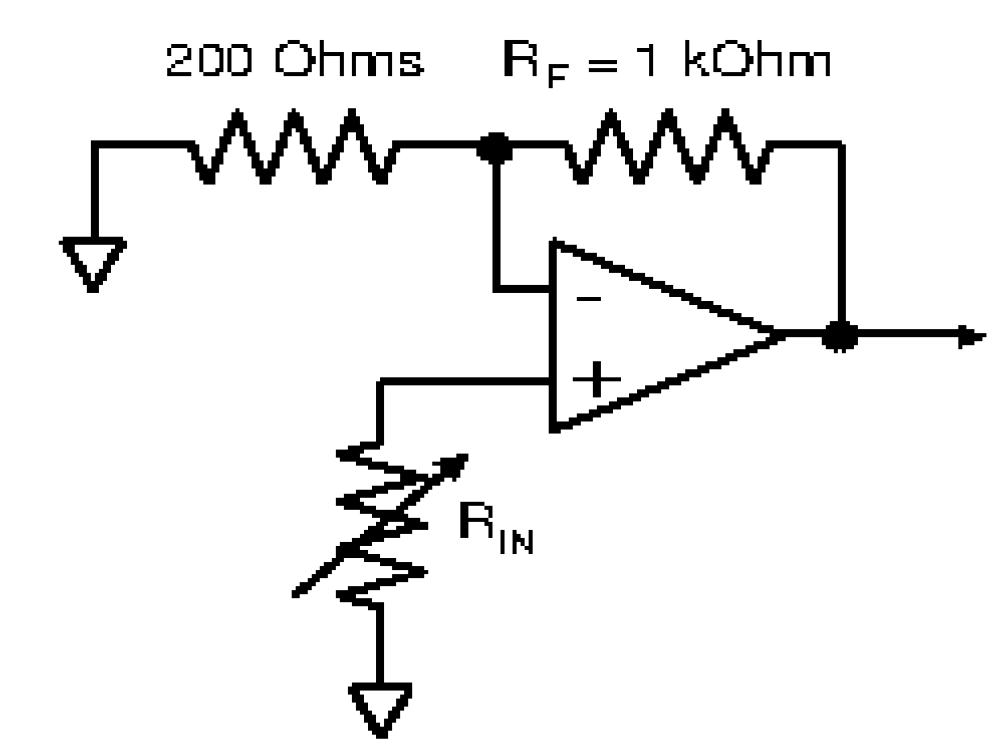
\includegraphics[width=0.5\textwidth]{figs/schalt amplifier.png}
    \caption{Schaltplan des Vorverstärkers der LLE-Box zur Messung des JohnsonRauschens \cite{praktikum}}
    \label{fig:schaltamplifier}
\end{figure}
\FloatBarrier

\FloatBarrier
\begin{figure}[htbp]
    \centering
    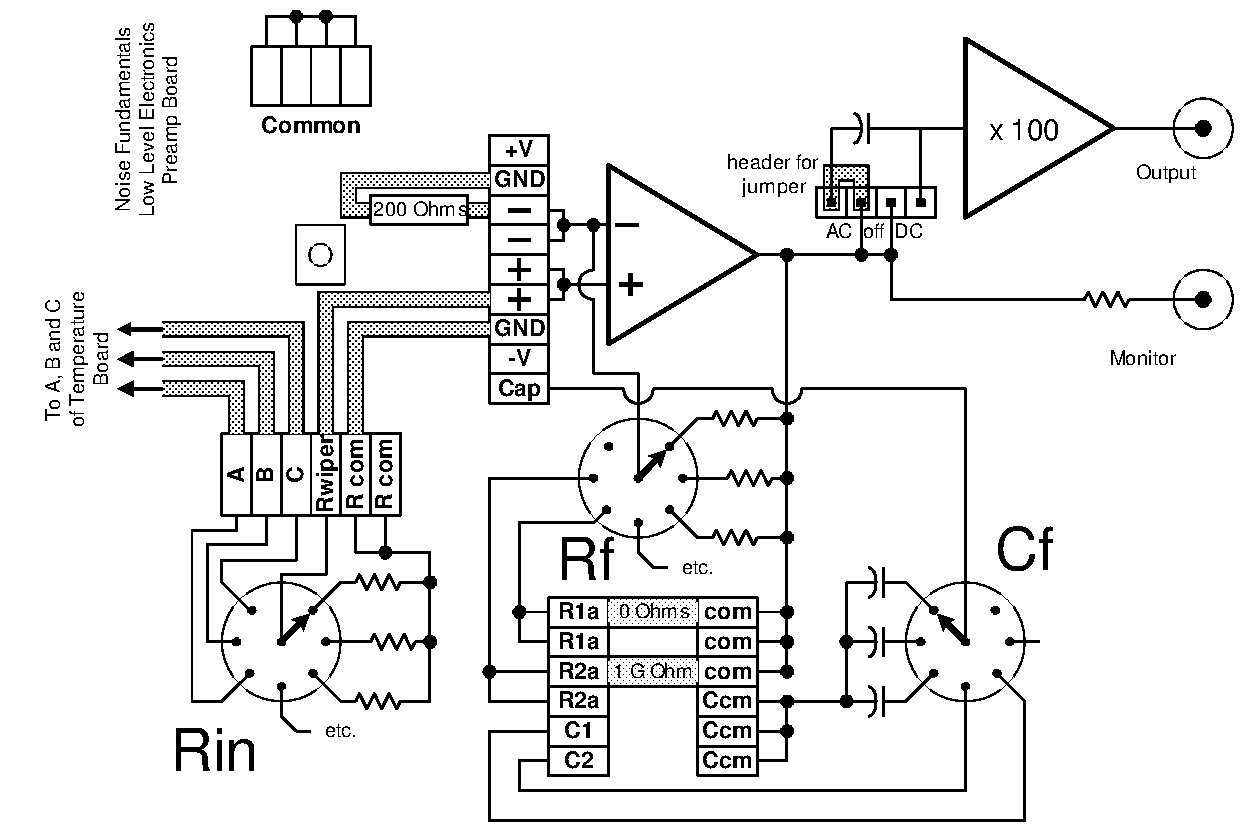
\includegraphics[width=0.75\textwidth]{figs/johnson lle.png}
    \caption{Interner Schaltplan der LLE-Box zur Messung des Johnson-Rauschens \cite{praktikum}}
    \label{fig:johnson lle}
\end{figure}
\FloatBarrier

\FloatBarrier
\begin{figure}[htbp]
    \centering
    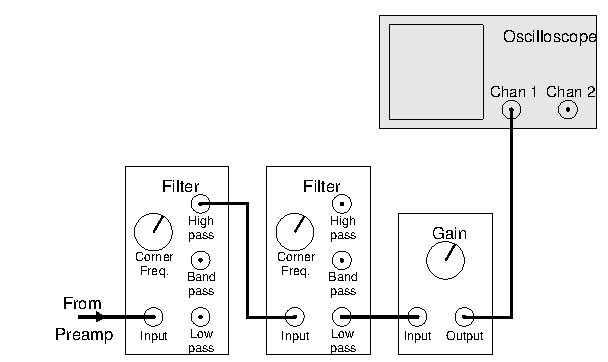
\includegraphics[width=0.5\textwidth]{figs/johnson hle.png}
    \caption{Schaltung der HLE-Box zum Visualisieren des Johnson-Rauschens \cite{praktikum}}
    \label{fig:johnson hle}
\end{figure}
\FloatBarrier
%==============================================================================================================================================================================================================
\section{Messung des Johnson-Rauschens}

\FloatBarrier
\begin{figure}[htbp]
    \centering
    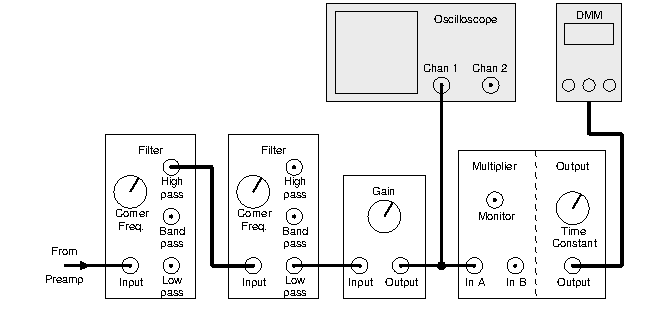
\includegraphics[width=0.5\textwidth]{figs/johnson hle and dmm.png}
    \caption{Verkabelung zur Messung des Johnson-Rauschens \cite{praktikum}}
    \label{fig:johnson messung}
\end{figure}
\FloatBarrier
